% answers.tex —— 2002 年·苏豫粤桂卷 · 参考答案与详细解析片段
% 由 tools/generate_projects.py 依来源总账自 2002/2002_数学真题_苏豫粤桂_试题.md + 2002/2002_数学真题_苏豫粤桂_解析正文.md + 2002/2002_数学真题_苏豫粤桂_答案要点.md 生成，勿手改（改源 MD 后重跑）


\begin{gktip}
固定 PDF 只有题面页，没有答案或评分页。以下解析是本库独立推导，不代表来源印载答案或官方解答；来源发布者、版次、复制/扫描链和身份未核，官方答案未认证。该 PDF 作为本库这套题面的 canonical 固定来源登记；这不认证其上游出版者、版次、复制链或官方身份。
\end{gktip}

\gkpart{一、选择题}

\begin{answer}
\gksolhead{1}{}

\textbf{题目}：

\Needspace{5\baselineskip}
函数
\nopagebreak[4]
\[
f(x)=\frac{\sin 2x}{\cos x}
\]
的最小正周期是\mbox{（　　）}

(A) $\dfrac{\pi}{2}$　　(B) $\pi$　　(C) $2\pi$　　(D) $4\pi$

\Needspace{4\baselineskip}
\textbf{解析}

在原定义域 $\cos x\ne0$ 上，$f(x)=2\sin x$。若 $T$ 是原函数的周期，定义域排除点集合也必须在平移 $T$ 后不变，这要求 $T$ 是 $\pi$ 的整数倍；又 $f(x+\pi)=-f(x)$，所以 $T$ 不能是 $\pi$ 的奇数倍。最小正周期是 $2\pi$，选 C。

\gkanswer{答案：C。}

\end{answer}
\begin{answer}
\gksolhead{2}{}

\textbf{题目}：

圆 $(x-1)^2+y^2=1$ 的圆心到直线 $y=\dfrac{\sqrt3}{3}x$ 的距离是\mbox{（　　）}

(A) $\dfrac12$　　(B) $\dfrac{\sqrt3}{2}$　　(C) $1$　　(D) $\sqrt3$

\Needspace{4\baselineskip}
\textbf{解析}

\Needspace{5\baselineskip}
圆心是 $(1,0)$。直线写作 $x-\sqrt3y=0$，圆心到直线的距离为
\nopagebreak[4]
\[
\frac{|1-\sqrt3\cdot0|}{\sqrt{1+3}}=\frac12,
\]
选 A。

\gkanswer{答案：A。}

\end{answer}
\begin{answer}
\gksolhead{3}{}

\textbf{题目}：

不等式 $(1+x)(1-|x|)>0$ 的解集是\mbox{（　　）}

(A) $\{x\mid 0\leqslant x<1\}$　　(B) $\{x\mid x<0\text{ \text{且} }x\ne-1\}$

(C) $\{x\mid -1<x<1\}$　　(D) $\{x\mid x<1\text{ \text{且} }x\ne-1\}$

\Needspace{4\baselineskip}
\textbf{解析}

当 $x<-1$ 时，$1+x<0$ 且 $1-|x|=1+x<0$，乘积为正；当 $-1<x<1$ 时两个因子均为正；$x=-1$ 使乘积为零，$x\geqslant1$ 时乘积不为正。因此解集为 $x<1$ 且 $x\ne-1$，选 D。

\gkanswer{答案：D。}

\end{answer}
\begin{answer}
\gksolhead{4}{}

\textbf{题目}：

在 $(0,2\pi)$ 内，使 $\sin x>\cos x$ 成立的 $x$ 的取值范围是\mbox{（　　）}

(A) $\left(\dfrac\pi4,\dfrac\pi2\right)\cup\left(\pi,\dfrac{5\pi}4\right)$

(B) $\left(\dfrac\pi4,\pi\right)$

(C) $\left(\dfrac\pi4,\dfrac{5\pi}4\right)$

(D) $\left(\dfrac\pi4,\pi\right)\cup\left(\dfrac{5\pi}4,\dfrac{3\pi}2\right)$

\Needspace{4\baselineskip}
\textbf{解析}

\nopagebreak[4]
\[
\sin x-\cos x=\sqrt2\sin\left(x-\frac\pi4\right).
\]
在 $0<x<2\pi$ 内令此式为正，得 $\pi/4<x<5\pi/4$，选 C。

\gkanswer{答案：C。}

\end{answer}
\begin{answer}
\gksolhead{5}{}

\textbf{题目}：

\Needspace{5\baselineskip}
设集合
\nopagebreak[4]
\[
M=\left\{x\middle|x=\frac{k}{2}+\frac14,\ k\in\mathbb Z\right\},\qquad
N=\left\{x\middle|x=\frac{k}{4}+\frac12,\ k\in\mathbb Z\right\},
\]
则\mbox{（　　）}

(A) $M=N$　　(B) $M\subseteq N$　　(C) $M\supseteq N$　　(D) $M\cap N=\varnothing$

\Needspace{4\baselineskip}
\textbf{解析}

集合 $M$ 中元素可写为 $(2k+1)/4$，是分子为奇整数的四分之一倍数；集合 $N$ 可写为 $(k+2)/4$，即所有整数的四分之一倍数。因此 $M\subseteq N$，选 B。

\gkanswer{答案：B。}

\end{answer}
\begin{answer}
\gksolhead{6}{}

\textbf{题目}：

一个圆锥和一个半球有公共底面，如果圆锥的体积恰好与半球的体积相等，那么这个圆锥轴截面顶角的余弦值是\mbox{（　　）}

(A) $\dfrac34$　　(B) $\dfrac45$　　(C) $\dfrac35$　　(D) $-\dfrac35$

\Needspace{4\baselineskip}
\textbf{解析}

\Needspace{5\baselineskip}
设圆锥与半球的公共底面半径为 $r$，圆锥高为 $h$。体积相等给出
\nopagebreak[4]
\[
\frac13\pi r^2h=\frac23\pi r^3,\qquad h=2r.
\]
\Needspace{5\baselineskip}
从圆锥顶点指向轴截面底边两端的向量夹角为顶角。其余弦为
\nopagebreak[4]
\[
\frac{h^2-r^2}{h^2+r^2}=\frac35,
\]
选 C。

\gkanswer{答案：C。}

\end{answer}
\begin{answer}
\gksolhead{7}{}

\textbf{题目}：

函数 $f(x)=x|x+a|+b$ 是奇函数的充要条件是\mbox{（　　）}

(A) $ab=0$　　(B) $a+b=0$　　(C) $a=b$　　(D) $a^2+b^2=0$

\Needspace{4\baselineskip}
\textbf{解析}

\Needspace{5\baselineskip}
奇函数必须满足 $f(0)=b=0$。再令 $f(x)+f(-x)=0$，对任意 $x$ 有
\nopagebreak[4]
\[
x\bigl(|x+a|-|x-a|\bigr)=0.
\]
若 $a\ne0$，取充分大的正 $x$，则 $|x+a|-|x-a|=2a\ne0$，矛盾；故 $a=0$。反之 $x|x|$ 是奇函数。因而 $a=b=0$，选 D。

\gkanswer{答案：D。}

\end{answer}
\begin{answer}
\gksolhead{8}{}

\textbf{题目}：

已知 $0<x<y<a<1$，则有\mbox{（　　）}

(A) $\log_a(xy)<0$　　(B) $0<\log_a(xy)<1$

(C) $1<\log_a(xy)<2$　　(D) $\log_a(xy)>2$

\Needspace{4\baselineskip}
\textbf{解析}

\Needspace{5\baselineskip}
由 $0<x<y<a$ 得 $0<xy<a^2$。因 $0<a<1$，函数 $\log_a t$ 严格递减，所以
\nopagebreak[4]
\[
\log_a(xy)>\log_a(a^2)=2.
\]
选 D。

\gkanswer{答案：D。}

\end{answer}
\begin{answer}
\gksolhead{9}{}

\textbf{题目}：

\Needspace{5\baselineskip}
函数
\nopagebreak[4]
\[
y=1-\frac{1}{x-1}
\]
\mbox{（　　）}

(A) 在 $(-1,+\infty)$ 内单调递增　　(B) 在 $(-1,+\infty)$ 内单调递减

(C) 在 $(1,+\infty)$ 内单调递增　　(D) 在 $(1,+\infty)$ 内单调递减

\Needspace{4\baselineskip}
\textbf{解析}

\Needspace{5\baselineskip}
在 $(1,+\infty)$ 上
\nopagebreak[4]
\[
y'=\frac1{(x-1)^2}>0,
\]
故函数严格递增，选 C。

\gkanswer{答案：C。}

\end{answer}
\begin{answer}
\gksolhead{10}{}

\textbf{题目}：

极坐标方程 $\rho=\cos\theta$ 与 $\rho\cos\theta=\dfrac12$ 的图形是\mbox{（　　）}

\textbf{原页图位：}四个选项图按固定来源重绘；(B) 中的竖线是 $x=\dfrac12$，不是 $y$ 轴。
\nopagebreak[4]
\begin{center}% 第 10 题四个极坐标图形选项，按固定来源第 1 页重绘。
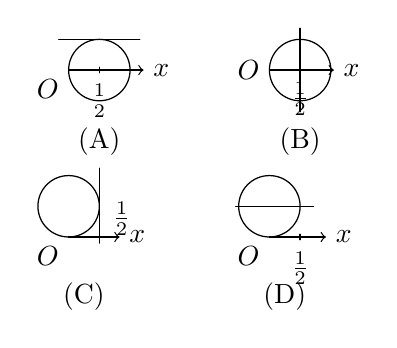
\begin{tikzpicture}[x=0.78cm,y=0.78cm,line width=0.45pt,line cap=round]
  % (A) rho=cos(theta) 对应圆心 (1/2,0)、半径 1/2；上方水平线相切。
  \begin{scope}
    \draw (0.5,0) circle (0.5);
    \draw (-0.16,0.5) -- (1.16,0.5);
    \draw[->] (0,0) -- (1.22,0) node[right] {$x$};
    \node[below left] at (0,0) {$O$};
    \draw (0.5,-0.045) -- (0.5,0.045);
    \node[below] at (0.5,-0.07) {$\frac12$};
    \node[below] at (0.5,-0.78) {(A)};
  \end{scope}

  % (B) 同一圆，x=1/2 直线通过圆心。
  \begin{scope}[xshift=2.55cm]
    \draw (0.5,0) circle (0.5);
    \draw (0.5,-0.68) -- (0.5,0.68);
    \draw[->] (0,0) -- (1.05,0) node[right] {$x$};
    \node[left] at (0,0) {$O$};
    \node[below] at (0.5,-0.04) {$\frac12$};
    \node[below] at (0.5,-0.78) {(B)};
  \end{scope}

  % (C) 干扰图：圆底端为 O，右侧竖线与圆相切。
  \begin{scope}[yshift=-2.12cm]
    \draw (0,0.5) circle (0.5);
    \draw (0.5,-0.10) -- (0.5,1.12);
    \draw[->] (0,0) -- (0.83,0) node[right] {$x$};
    \node[below left] at (0,0) {$O$};
    \node[right] at (0.56,0.30) {$\frac12$};
    \node[below] at (0.25,-0.58) {(C)};
  \end{scope}

  % (D) 干扰图：圆底端为 O，水平线通过圆心。
  \begin{scope}[xshift=2.55cm,yshift=-2.12cm]
    \draw (0,0.5) circle (0.5);
    \draw (-0.55,0.5) -- (0.72,0.5);
    \draw[->] (0,0) -- (0.92,0) node[right] {$x$};
    \node[below left] at (0,0) {$O$};
    \draw (0.5,-0.045) -- (0.5,0.045);
    \node[below] at (0.5,-0.08) {$\frac12$};
    \node[below] at (0.25,-0.58) {(D)};
  \end{scope}
\end{tikzpicture}
\end{center}
\nopagebreak[4]
\Needspace{4\baselineskip}
\textbf{解析}

\Needspace{5\baselineskip}
由 $\rho=\cos\theta$ 乘以 $\rho$，并用 $x=\rho\cos\theta$、$x^2+y^2=\rho^2$，得
\nopagebreak[4]
\[
x^2+y^2=x,
\]
即圆心 $(1/2,0)$、半径 $1/2$ 的圆。另一式 $\rho\cos\theta=1/2$ 即直线 $x=1/2$，它是圆的竖直直径线。与原页选项图对照为 B。原页 B 的原点 $O$ 位于圆左端，竖线不是 $y$ 轴。

\gkanswer{答案：B。}

\end{answer}
\begin{answer}
\gksolhead{11}{}

\textbf{题目}：

从正方体的 6 个面中选取 3 个面，其中有 2 个面不相邻的选法共有\mbox{（　　）}

(A) 8 种　　(B) 12 种　　(C) 16 种　　(D) 20 种

\Needspace{4\baselineskip}
\textbf{解析}

\Needspace{5\baselineskip}
先从正方体的三对相对面中选一对，再从其余四面中任选一面，共
\nopagebreak[4]
\[
3\times4=12
\]
种，选 B。

\gkanswer{答案：B。}

\end{answer}
\begin{answer}
\gksolhead{12}{}

\textbf{题目}：

据 2002 年 3 月 5 日九届人大五次会议《政府工作报告》：“2001 年国内生产总值达到 95933 亿元，比上年增长 7.3\%”，如果“十·五”期间（2001 年—2005 年）每年的国内生产总值都按此年增长率增长，那么到“十·五”末我国国内年生产总值约为\mbox{（　　）}

(A) 115000 亿元　　(B) 120000 亿元　　(C) 127000 亿元　　(D) 135000 亿元

\Needspace{4\baselineskip}
\textbf{解析}

\Needspace{5\baselineskip}
2001 年数值到 2005 年经历 4 个年度增长区间，故估算为
\nopagebreak[4]
\[
95933(1+0.073)^4\approx127000\quad(\text{亿元}),
\]
选 C。

\gkanswer{答案：C。}

\end{answer}
\gkpart{二、填空题}

\begin{answer}
\gksolhead{13}{}

\textbf{题目}：

椭圆 $5x^2+ky^2=5$ 的一个焦点是 $(0,2)$，那么 $k=\underline{\qquad}$。

\Needspace{4\baselineskip}
\textbf{解析}

\Needspace{5\baselineskip}
化为标准式 $x^2+y^2/(5/k)=1$。焦点位于 $y$ 轴且焦距参数 $c=2$，所以 $5/k>1$ 且
\nopagebreak[4]
\[
\frac5k-1=c^2=4,
\]
解得 $k=1$。

\gkanswer{答案：$1$。}

\end{answer}
\begin{answer}
\gksolhead{14}{}

\textbf{题目}：

$(x^2+1)(x-2)^7$ 展开式中 $x^3$ 的系数是$\underline{\qquad}$。

\Needspace{4\baselineskip}
\textbf{解析}

\Needspace{5\baselineskip}
所求系数来自 $x^2\cdot(x-2)^7$ 的 $x^1$ 项，以及 $(x-2)^7$ 的 $x^3$ 项：
\nopagebreak[4]
\[
\binom71(-2)^6+\binom73(-2)^4=448+560=1008.
\]

\gkanswer{答案：$1008$。}

\end{answer}
\begin{answer}
\gksolhead{15}{}

\textbf{题目}：

已知 $\sin\alpha=\cos2\alpha$，$\alpha\in\left(\dfrac\pi2,\pi\right)$，则 $\tan\alpha=\underline{\qquad}$。

\Needspace{4\baselineskip}
\textbf{解析}

\Needspace{5\baselineskip}
令 $s=\sin\alpha$。由 $\cos2\alpha=1-2s^2$ 得
\nopagebreak[4]
\[
2s^2+s-1=0,\qquad s=\frac12\text{ 或 }-1.
\]
因 $\alpha\in(\pi/2,\pi)$，取 $s=1/2$，于是 $\cos\alpha=-\sqrt3/2$，$\tan\alpha=-\sqrt3/3$。

\gkanswer{答案：$-\dfrac{\sqrt3}{3}$。}

\end{answer}
\begin{answer}
\gksolhead{16}{}

\textbf{题目}：

\Needspace{5\baselineskip}
已知 $f(x)=\dfrac{x^2}{1+x^2}$，那么
\nopagebreak[4]
\[f(1)+f(2)+f\left(\frac12\right)+f(3)+f\left(\frac13\right)+f(4)+f\left(\frac14\right)=\underline{\qquad}\text{。}\]

\Needspace{4\baselineskip}
\textbf{解析}

对任意非零 $x$，有 $f(x)+f(1/x)=1$。将三对倒数项 $(2,1/2)$、$(3,1/3)$、$(4,1/4)$ 配对，另 $f(1)=1/2$，故总和为 $3+1/2=7/2$。

\gkanswer{答案：$\dfrac72$。}

\end{answer}
\gkpart{三、解答题}

\begin{answer}
\gksolhead{17}{}

\textbf{题目}：

\Needspace{5\baselineskip}
已知复数 $z=1+i$，求实数 $a,b$ 使
\nopagebreak[4]
\[az+2b\overline{z}=(a+2z)^2\text{。}\]

\Needspace{4\baselineskip}
\textbf{解析}

\Needspace{5\baselineskip}
代入 $z=1+i$，得
\nopagebreak[4]
\[
(a+2b)+i(a-2b)=\bigl((a+2)+2i\bigr)^2.
\]
\Needspace{5\baselineskip}
比较实部与虚部：
\nopagebreak[4]
\[
a+2b=a^2+4a,\qquad a-2b=4a+8.
\]
两式相加得 $a^2+6a+8=0$，所以 $a=-2$ 或 $a=-4$。代回第二式，分别得 $b=-1$、$b=2$。答案为 $(-2,-1)$、$(-4,2)$。

\gkanswer{答案：$(a,b)=(-2,-1)$ 或 $(-4,2)$。}

\end{answer}
\begin{answer}
\gksolhead{18}{}

\textbf{题目}：

设 $\{a_n\}$ 为等差数列，$\{b_n\}$ 为等比数列，$a_1=b_1=1$，$a_2+a_4=b_3$，$b_2b_4=a_3$，分别求出 $\{a_n\}$ 及 $\{b_n\}$ 的前 10 项的和 $S_{10}$ 及 $T_{10}$。

\Needspace{4\baselineskip}
\textbf{解析}

\Needspace{5\baselineskip}
设等差公差为 $d$、等比公比为 $q$。由题设
\nopagebreak[4]
\[
2+4d=q^2,\qquad 1+2d=q^4.
\]
令 $t=q^2\geqslant0$，消去 $d$ 得 $t^2=t/2$，故 $t=0$ 或 $t=1/2$。

\begin{itemize}
\item 若允许 $q=0$，则 $d=-1/2$，$S_{10}=5(2+9d)=-25/2$，且等比数列为 $1,0,\ldots$，$T_{10}=1$。
\item 若 $q=\pm1/\sqrt2$，则 $d=-3/8$，$S_{10}=5(2+9d)=-55/8$。并且
\end{itemize}
\nopagebreak[4]
\[
  T_{10}=\frac{1-q^{10}}{1-q}=\begin{cases}
  \dfrac{31(2+\sqrt2)}{32},&q=1/\sqrt2,\\[3pt]
  \dfrac{31(2-\sqrt2)}{32},&q=-1/\sqrt2.
  \end{cases}
\]

题面只说“等比数列”，未见来源答案或约定说明零公比是否允许，故两种常见定义口径都保留，不擅自删去 $q=0$ 分支。

\gkanswer{答案：U/PENDING。}

\end{answer}
\begin{answer}
\gksolhead{19}{}

\textbf{题目}：

四棱锥 $P-ABCD$ 的底面是边长为 $a$ 的正方形，$PB\perp$ 平面 $ABCD$。

(1) 若面 $PAD$ 与面 $ABCD$ 所成的二面角为 $60^\circ$，求这个四棱锥的体积；

(2) 证明无论四棱锥的高怎样变化，面 $PAD$ 与面 $PCD$ 所成的二面角恒大于 $90^\circ$。

\textbf{原页图位：}四棱锥示意图标出顶点 $P,A,B,C,D$；底面边 $AB$、$BC$ 为虚线，$PB$ 为虚线，$PA$、$PC$、$PD$、$AD$、$CD$ 为实线。
\nopagebreak[4]
\begin{center}% 第 19 题四棱锥示意图，虚实线按固定来源第 1 页重绘；坐标仅控制图形布局。
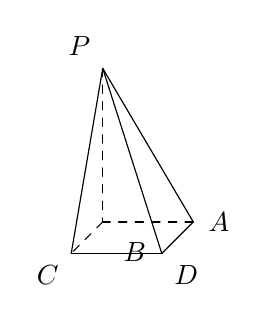
\begin{tikzpicture}[x=1cm,y=1cm,line width=0.42pt,line cap=round,line join=round]
  \coordinate (B) at (0,0);
  \coordinate (A) at (1.15,0);
  \coordinate (C) at (-0.40,-0.40);
  \coordinate (D) at (0.75,-0.40);
  \coordinate (P) at (0,1.95);

  % 虚线：PB、AB、BC。
  \draw[dashed] (P) -- (B);
  \draw[dashed] (A) -- (B);
  \draw[dashed] (B) -- (C);

  % 实线：PA、PC、PD、AD、CD。
  \draw (P) -- (A);
  \draw (P) -- (C);
  \draw (P) -- (D);
  \draw (A) -- (D);
  \draw (C) -- (D);

  \node[above left=1pt] at (P) {$P$};
  \node[right=2pt] at (A) {$A$};
  \node[below right=4pt] at (B) {$B$};
  \node[below left=1pt] at (C) {$C$};
  \node[below right=1pt] at (D) {$D$};
\end{tikzpicture}
\end{center}
\nopagebreak[4]
\Needspace{4\baselineskip}
\textbf{解析}

\Needspace{5\baselineskip}
取坐标
\nopagebreak[4]
\[
A=(0,0,0),\ B=(a,0,0),\ C=(a,a,0),\ D=(0,a,0),\ P=(a,0,h).
\]

\gksubpart{(1) 求体积}

\Needspace{5\baselineskip}
(1) $AD$ 的方向为 $y$ 轴方向。$AB$ 与 $AP$ 都垂直于 $AD$，截面内的角 $\angle BAP$ 就是所给二面角，因此 $\tan60^\circ=h/a$，即 $h=\sqrt3a$。所以
\nopagebreak[4]
\[
V=\frac13a^2h=\frac{\sqrt3}{3}a^3.
\]

\gksubpart{(2) 证明二面角恒大于 $90^\circ$}

\Needspace{5\baselineskip}
(2) 按四棱锥两侧面沿公共棱围成的内二面角理解。公共棱方向向量取 $w=P-D=(a,-a,h)$；两面内垂直于公共棱的方向分别由 $u=A-D=(0,-a,0)$、$v=C-D=(a,0,0)$ 投影得到。投影内积为
\nopagebreak[4]
\[
u\cdot v-\frac{(u\cdot w)(v\cdot w)}{|w|^2}
=-\frac{a^4}{2a^2+h^2}<0.
\]
两投影所成角为钝角，故两面沿 $PD$ 所成的内二面角恒大于 $90^\circ$。

\gkanswer{答案（1）：$V=\dfrac{\sqrt3}{3}a^3$。}

\gkanswer{答案（2）：按棱锥两侧面沿公共棱围成的内二面角理解，恒大于 $90^\circ$。}

\end{answer}
\begin{answer}
\gksolhead{20}{}

\textbf{题目}：

\Needspace{5\baselineskip}
设 $A\text{、}B$ 是双曲线
\nopagebreak[4]
\[
x^2-\frac{y^2}{2}=1
\]
上的两点，点 $N(1,2)$ 是线段 $AB$ 的中点。

(1) 求直线 $AB$ 的方程；

(2) 如果线段 $AB$ 的垂直平分线与双曲线相交于 $C\text{、}D$ 两点，那么 $A\text{、}B\text{、}C\text{、}D$ 四点是否共圆？为什么？

\Needspace{4\baselineskip}
\textbf{解析}

\gksubpart{(1) 求弦方程}

\Needspace{5\baselineskip}
若 $AB$ 竖直，则其方程为 $x=1$；代入双曲线仅有一个交点 $(1,0)$，不可能得到中点为 $N=(1,2)$ 的两个不同端点。因此设 $AB$ 的方向向量为 $(1,m)$。因 $N$ 是弦中点，可将两交点写成
\nopagebreak[4]
\[
A=N+t(1,m),\qquad B=N-t(1,m),\qquad t\ne0.
\]
代入双曲线，关于参数 $t$ 的一次项系数为 $2(1-m)$。两端点对应 $t$、$-t$ 都在曲线上，因此该系数为零，得 $m=1$，即 $AB:y=x+1$。与双曲线联立得 $A=(3,4)$、$B=(-1,0)$。

\gksubpart{(2) 判断四点共圆}

\Needspace{5\baselineskip}
其垂直平分线为 $x+y=3$。与双曲线相交得到
\nopagebreak[4]
\[
C,D=(-3\pm2\sqrt5,\ 6\mp2\sqrt5).
\]
\Needspace{5\baselineskip}
取圆心 $O=(-3,6)$，则
\nopagebreak[4]
\[
OA^2=OB^2=40,
\qquad OC^2=OD^2=(2\sqrt5)^2+(-2\sqrt5)^2=40.
\]
所以四点共圆，圆方程为 $(x+3)^2+(y-6)^2=40$。注意圆心不是弦中点 $N$。

\gkanswer{答案（1）：$y=x+1$。}

\gkanswer{答案（2）：四点共圆，圆心 $(-3,6)$，半径 $2\sqrt{10}$。}

\end{answer}
\begin{answer}
\gksolhead{21}{}

\textbf{题目}：

(1) 给出两块相同的正三角形纸片（如图 1、图 2），要求用其中一块剪拼成一个三棱锥模型，另一块剪拼成一个正三棱柱模型，使它们的全面积都与原三角形的面积相等。请设计一种剪拼方法，分别用虚线标示在图 1、图 2 中，并作简要说明；

(2) 试比较你剪拼的正三棱锥与正三棱柱的体积的大小；

(3) 如果给出的是一块任意三角形的纸片（如图 3），要求剪拼成一个直三棱柱，使它的全面积与给出的三角形的面积相等。请设计一种剪拼方法，用虚线标示在图 3 中，并作简要说明。

\textbf{原页图位：}图 1、图 2 为两块相同正三角形轮廓，图 3 为任意三角形轮廓；原图没有剪切虚线，供作答者自行标示。
\nopagebreak[4]
\begin{center}% 第 21 题原页图：只重绘三块空白三角形轮廓；原卷没有预印剪线。
\begin{tikzpicture}[x=0.78cm,y=0.78cm,line cap=round,line join=round,
  outline/.style={draw=black,line width=0.55pt}]
  % 图 1、图 2：正三角形轮廓。
  \draw[outline] (1,1.732) -- (0,0) -- (2,0) -- cycle;
  \node[below=2pt] at (1,-0.03) {图 1};

  \begin{scope}[xshift=2.35cm]
    \draw[outline] (1,1.732) -- (0,0) -- (2,0) -- cycle;
    \node[below=2pt] at (1,-0.03) {图 2};
  \end{scope}

  % 图 3：按原页比例重绘任意三角形示意轮廓。
  \begin{scope}[xshift=4.75cm]
    \draw[outline] (0.75,1.75) -- (0,0) -- (4,0) -- cycle;
    \node[below=2pt] at (2,-0.03) {图 3};
  \end{scope}
\end{tikzpicture}
\end{center}
\nopagebreak[4]
\Needspace{4\baselineskip}
\textbf{解析}
\nopagebreak[4]
\begin{center}% 第 21 题答案辅助图：虚线仅标示原纸片剪线，不表示剪下后的拼合状态。
% 数字 1、2 标出所选的两块三角形底面；侧面配对与平移步骤见解析正文。
\begin{tikzpicture}[x=0.78cm,y=0.78cm,line cap=round,line join=round,
  outline/.style={draw=black,line width=0.65pt},
  cut/.style={draw=black,line width=0.55pt,densely dashed},
  font=\scriptsize]
  % 图 1：中点剪线将正三角形分成四个全等小三角形。
  \draw[outline] (1,1.732) -- (0,0) -- (2,0) -- cycle;
  \draw[cut]
    (0.5,0.866) -- (1.5,0.866)
    (0.5,0.866) -- (1,0)
    (1.5,0.866) -- (1,0);
  \node[below=2pt] at (1,-0.03) {图 1};

  % 图 2：中点剪线后，另两块角三角形再按内心—顶点连线切分。
  \begin{scope}[xshift=2.35cm]
    \draw[outline] (1,1.732) -- (0,0) -- (2,0) -- cycle;
    \draw[cut]
      (0.5,0.866) -- (1.5,0.866)
      (0.5,0.866) -- (1,0)
      (1.5,0.866) -- (1,0)
      (0.5,0.289) -- (0,0)
      (0.5,0.289) -- (0.5,0.866)
      (0.5,0.289) -- (1,0)
      (1.5,0.289) -- (2,0)
      (1.5,0.289) -- (1.5,0.866)
      (1.5,0.289) -- (1,0);
    \node at (1,0.58) {1};
    \node at (1,1.16) {2};
    \node[below=2pt] at (1,-0.03) {图 2};
  \end{scope}

  % 图 3：近似源图轮廓；两块底面与图 2 采用相同位置关系。
  \begin{scope}[xshift=4.75cm]
    \coordinate (A) at (0.75,1.75);
    \coordinate (B) at (0,0);
    \coordinate (C) at (4,0);
    \coordinate (Mab) at (0.375,0.875);
    \coordinate (Mac) at (2.375,0.875);
    \coordinate (Mbc) at (2,0);
    \coordinate (IL) at (0.553,0.365);
    \coordinate (IR) at (2.553,0.365);

    \draw[outline] (A) -- (B) -- (C) -- cycle;
    \draw[cut]
      (Mab) -- (Mac)
      (Mab) -- (Mbc)
      (Mac) -- (Mbc)
      (IL) -- (B)
      (IL) -- (Mab)
      (IL) -- (Mbc)
      (IR) -- (C)
      (IR) -- (Mac)
      (IR) -- (Mbc);
    \node at (1.583,0.583) {1};
    \node at (1.25,1.167) {2};
    \node[below=2pt] at (2,-0.03) {图 3};
  \end{scope}
\end{tikzpicture}
\end{center}
\nopagebreak[4]
\gksubpart{(1) 正三棱锥与正三棱柱剪拼}

(1) 设给定正三角形边长为 $L$，连接三边中点，将其分成四个边长 $s=L/2$ 的全等正三角形。

\begin{itemize}
\item \textbf{正三棱锥：}取中央小三角形作底面，三个角上的小三角形作侧面，沿底面三边折起即得正四面体。每个面面积是原纸片面积的 $1/4$，总表面积正好等于原面积。
\item \textbf{正三棱柱：}取其中两块作两个正三角形底面。另两块各连结内心与三个顶点，得到对应的三对小三角形。对每条底边，将两块对应小三角形沿一条对应的内心—顶点边反向拼合，组成以该底边为一组对边的平行四边形；其底边长 $s$、高为小正三角形内切圆半径 $r=\sqrt3s/6$。在这个平行四边形中，斜边沿底边方向的错位小于 $s$（等边情形为 $s/2$）。从一端底角向上作垂线剪开，取外侧直角三角形平移到另一端补齐，即得 $s\times r$ 矩形。三块矩形接成侧面条带，再接上两个三角形底面，构成正三棱柱展开图。总面积为
\end{itemize}
\nopagebreak[4]
\[
  2\cdot\frac{\sqrt3}{4}s^2+3sr
  =\frac{\sqrt3}{2}s^2+\frac{\sqrt3}{2}s^2
  =\sqrt3s^2=\frac{\sqrt3}{4}L^2,
\]
  等于原正三角形面积。

\gksubpart{(2) 比较体积}

\Needspace{5\baselineskip}
(2) 四面体棱长为 $s$，故
\nopagebreak[4]
\[
V_{\rm tetra}=\frac{\sqrt2}{12}s^3.
\]
\Needspace{5\baselineskip}
棱柱高为 $r=\sqrt3s/6$，故
\nopagebreak[4]
\[
V_{\rm prism}=\frac{\sqrt3}{4}s^2\cdot\frac{\sqrt3}{6}s=\frac18s^3.
\]
由于 $1/8>\sqrt2/12$，该剪拼的正三棱柱体积较大。

\gksubpart{(3) 任意三角形剪拼成直三棱柱}

\Needspace{5\baselineskip}
(3) 设原任意三角形面积为 $A$。仍连接三边中点，得到四个全等小三角形，各面积 $K=A/4$；取两块作底面，另两块各用内心到顶点的线分成三块。对小三角形的每条边 $c_i$，把两份对应小三角形沿对应内心—顶点边反向拼成平行四边形，其一组对边长为 $c_i$，高为小三角形内切圆半径 $r$。内心到该边的垂足在边段内部，故平行四边形的横向错位小于 $c_i$；可从一端向上作垂线剪下外侧三角形，平移至另一端，得到 $c_i\times r$ 矩形。三矩形作直三棱柱侧面，棱柱高为 $r$。小三角形周长记 $p$，则 $K=pr/2$；表面积
\nopagebreak[4]
\[
2K+pr=4K=A.
\]
所以所得直三棱柱的全面积等于原任意三角形面积。

\gkanswer{答案（1）：连接正三角形三边中点分成四块；一块作正四面体底面，另三块作侧面。另一张纸也按中点分割，选两块作棱柱底面，其余两块按内心至顶点分割并配对、剪角平移成三个矩形侧面。}

\gkanswer{答案（2）：本构造下正三棱柱体积较大，$V_{\rm prism}=s^3/8>V_{\rm tetra}=\sqrt2s^3/12$。}

\gkanswer{答案（3）：任意三角形仍按三边中点分成四块，选两块作底面；其余两块由内心至顶点分割，配对并剪角平移为等高矩形侧面，构成直三棱柱。}

\end{answer}
\begin{answer}
\gksolhead{22}{}

\textbf{题目}：

已知 $a>0$，函数 $f(x)=ax-bx^2$。

(1) 当 $b>0$ 时，若对任意 $x\in\mathbb R$ 都有 $f(x)\leqslant1$，证明：$a\leqslant2\sqrt b$；

(2) 当 $b>1$ 时，证明：对任意 $x\in[0,1]$，$|f(x)|\leqslant1$ 的充要条件是 $b-1\leqslant a\leqslant2\sqrt b$；

(3) 当 $0<b\leqslant1$ 时，讨论：对任意 $x\in[0,1]$，$|f(x)|\leqslant1$ 的充要条件。

\Needspace{4\baselineskip}
\textbf{解析}

\gksubpart{(1) 当 $b>0$ 时}

\Needspace{5\baselineskip}
(1) $b>0$ 时抛物线开口向下，最大值在 $x=a/(2b)$ 处，且
\nopagebreak[4]
\[
\max_{x\in\mathbb R}f(x)=\frac{a^2}{4b}\leqslant1.
\]
因 $a,b>0$，得 $a\leqslant2\sqrt b$。

\gksubpart{(2) 当 $b>1$ 时}

\Needspace{5\baselineskip}
(2) $b>1$ 时，$f$ 为开口向下的抛物线，区间最小值在端点，条件 $f(1)=a-b\geqslant-1$ 即 $a\geqslant b-1$。若顶点在 $[0,1]$，则最大值 $a^2/(4b)\leqslant1$ 等价于 $a\leqslant2\sqrt b$。若顶点在区间右侧，即 $a>2b$，函数在 $[0,1]$ 上递增，最大值条件要求 $a-b\leqslant1$，与 $a>2b$ 和 $b>1$ 矛盾。因此充要条件为
\nopagebreak[4]
\[
b-1\leqslant a\leqslant2\sqrt b.
\]
此范围内 $2\sqrt b<2b$，故顶点确在区间内，且端点最小值不少于 $-1$，条件也充分。

\gksubpart{(3) 当 $0<b\leqslant1$ 时}

\Needspace{5\baselineskip}
(3) $0<b\leqslant1$ 时，$f(1)=a-b>-b\geqslant-1$，下界自动满足。若 $a\leqslant2b$，顶点在区间内，最大值 $a^2/(4b)\leqslant b\leqslant1$；若 $a>2b$，函数在区间递增，最大值为 $a-b$，上界条件是 $a\leqslant b+1$。合并两种情形，充要条件为
\nopagebreak[4]
\[
0<a\leqslant b+1.
\]

\gkanswer{答案（1）：$a\leqslant2\sqrt b$。}

\gkanswer{答案（2）：$b-1\leqslant a\leqslant2\sqrt b$。}

\gkanswer{答案（3）：$0<a\leqslant b+1$。}

\end{answer}